% \section{Мотивация}

\subsection{Относительные вероятности распада}\label{branchings}

Наиболее точные измерения процесса $e^+e^-\to\pi^0\gamma$ проведены в
экспериментах на $e^+e^-$ коллайдере ВЭПП-2М с детекторами КМД-2 и СНД.
Из этих данных только распад $\omega (720) \to \pi^0\gamma$ был измерен с
относительно высокой точностью.
Распады $ \rho (770) $ и $ \phi (1020) $ и их возбуждённых состояний в $\pi^0\gamma$ главным образом требуют увеличения статистики.

\subsubsection{\texorpdfstring{$\omega \to \pi^0 \gamma$}{omega --> pi0 gamma}}
\label{omega-to-pi0-gamma}

Точность обобщённого результата КМД-2 и СНД произведения
$B( \omega \to \pi^0 \gamma ) \times B (\omega \to e^+ e^-) = \num{6.18 \pm 0.11 e-6} \, ( S
\footnote{Фактор масштабирования ошибок, используемый при усреднение или подгонки моделью набора данных, с целью компенсации противоречивости различных измерений.}
= 1.6 )$
составляет \SI{1.8}{\percent}.% .11/6.18 = 0.01779935275080906
Однако, это значение произведения отличается от
аналогичного, рассчитанного по $B( \omega \to \pi^0 \gamma )$ и
$B (\omega \to e^+ e^-)$, приведённых в таблице ПДГ \cite{Agashe:2014kda} (см. Рис.~\ref{fig:BweeXBwpig}).
\begin{figure}[htbp]
    \centering
    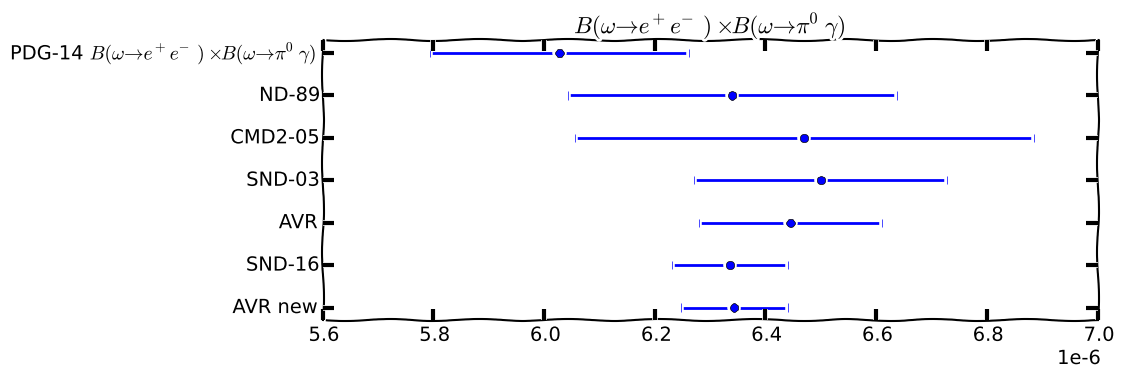
\includegraphics[width=.85\textwidth]{{img/Bw2ee_x_Bwpi0g}.png}
    \caption{$B(\omega \to e^+e^-) \times B(\omega \to \pi^0\gamma)$.
    PDG-14 --- \cite{Agashe:2014kda},
    ND-89 --- \cite{Dolinsky:1988zy},
    CMD2-05 --- \cite{Akhmetshin:2004gw},
    SND-03 --- \cite{Achasov:2003ed},
    AVR --- среднее \cite{Dolinsky:1988zy, Akhmetshin:2004gw, Achasov:2003ed},
    SND-16 --- \cite{Achasov:2016bfr},
    AVR new --- среднее \cite{Dolinsky:1988zy, Akhmetshin:2004gw, Achasov:2016bfr}}
    \label{fig:BweeXBwpig}
\end{figure}
Эта разница вызвана существованием противоречием между измереными значениями
$B( \omega \to \pi^0 \gamma ) \times B(\omega \to e^+ e^-)$,
$B( \omega \to \pi^0 \gamma ) \times B (\omega \to \pi^+ \pi^- \pi^0)$ и
$B( \omega \to \pi^0 \gamma ) / B (\omega \to \pi^+ \pi^- \pi^0)$ (см. Рис.~\ref{fig:Gw2pi0g_o_Gw2pippimpi0}).
Два последних выражения известны с точностью \SI{1.6}{\percent} и \SI{1.8}{\percent} соответственно,
и определяют нынешнее значение $B( \omega \to \pi^0 \gamma )$,
приводимое ПДГ.
Для прояснения этого противоречия необходимо улучшение точности
измерения сечения $e^+e^- \to \pi^0\gamma$ в области $\omega$-резонанса.

\begin{figure}[htbp]
    \centering
    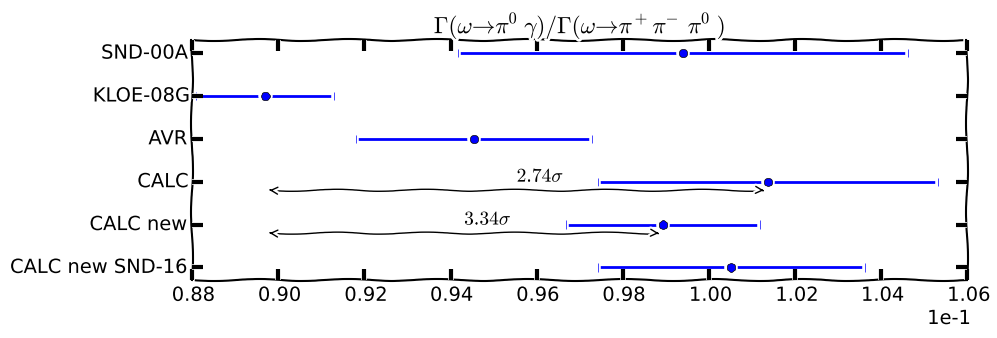
\includegraphics[width=.85\textwidth]{{img/Gw2pi0g_o_Gw2pippimpi0}.png}
    \caption{Отношение ширины распада $\omega \to \pi^0 \gamma$ к $\Gamma (\omega \to \pi^+ \pi^- \pi^0)$.
    SND-00A --- \cite{Aulchenko:2000zq},
    KLOE-08G --- \cite{Ambrosino:2008gb},
    AVR --- средние значение предыдущих двух,
    CALC --- среднее \cite{Akhmetshin:2004gw, Achasov:2003ed, Dolinsky:1988zy} делённое на среднее \cite{Akhmetshin:2003zn, Aubert:2004kj, Achasov:2003ir},
    CALC new --- среднее \cite{Akhmetshin:2004gw, Achasov:2016bfr, Dolinsky:1988zy} делённое на среднее \cite{Akhmetshin:2003zn, Aubert:2004kj, Achasov:2003ir},
    CALC new SND-16 --- \cite{Achasov:2016bfr} делённое на среднее \cite{Akhmetshin:2003zn, Aubert:2004kj, Achasov:2003ir}}
    \label{fig:Gw2pi0g_o_Gw2pippimpi0}
\end{figure}

\subsubsection{\texorpdfstring{$\rho \to \pi^0 \gamma$}{rho --> pi0 gamma}}
\label{rho-to-pi0-gamma}

Точность измерения относительной вероятности распада
$\rho \to \pi^0 \gamma$ составляет \SI{13}{\percent} и определяется статистикой
существующих измерений.

\subsubsection{\texorpdfstring{$\phi \to \pi^0 \gamma$}{}}
\label{phi-to-pi0-gamma}

Формальная точность значения ПДГ вероятности распада
$\phi \to \pi^0 \gamma$ лучше \SI{5}{\percent}.
Оно получено путём усреднения измерений \cite{Achasov:2000zd,Akhmetshin:2004gw} с систематической
ошибкой порядка \SI{8}{\percent} каждое.
Систематическая ошибка возникает из
неопределённости интерференции нерезонансной амплитуды с амплитудой
$\phi \to \pi^0 \gamma$ распада. Нерезонансная амплитуда определяется
вкладами хвостов резонансов $\omega$ и $\rho^0$, заодно дают вклад и
высшие возбуждения векторных мезонов.

Чтобы уменьшить неопределённость таких вкладов, необходимо улучшить
точность измерения сечения $e^+e^- \to \pi^0 \gamma$ в широком диапазоне
энергий от энергий \SI{\sim 300}{\MeVr} до \SI{2}{\GeVr}.

\subsection{Аномальный магнитный момент мюона}\label{mu-amm}

Как люди не могут забыть Герострата, сжёгшего храм Артемиды, так и физики
элементарных частиц рвутся попасть в истории кардинально изменив или
изничтожив современную парадигму науки --- Стандартную Модель. Некоторые
из них ищут Новую Физику пробуя другие области энергии и массы, кто-то
ищет новые распады, другие же могут мерить что-то очень точно и
сравнивать это с предсказаниями теории.
К последней группе относится изучение аномального магнитного момента мюона.

%%%%%%%%%%%%%%%%%%%%%%%%%%%%%%%%%%%%%%%%%%%%%%%%%%%%%%%%%%%%%%%%%%%%%%%%%%%%%%%%
\subsubsection{История}\label{g-2-history}

Экспериментальные измерения $a_\mu$ впервые было осуществлено в СЛАКе \cite{Garwin:1960zz}.
Затем последовала серия измерений в ЦЕРНе, уступившее свое место эксперементу в БНЛ.
В настоящий момент готовится два эксперимента по измерению $g_\mu-2$: в ФНАЛ \cite{Grange:2015fou} и Джей-ПАРКе \cite{Saito:2012zz}.


%%%%%%%%%%%%%%%%%%%%%%%%%%%%%%%%%%%%%%%%%%%%%%%%%%%%%%%%%%%%%%%%%%%%%%%%%%%%%%%%
\subsubsection{Вклады в \texorpdfstring{$g_\mu-2$}{muon g-2}}
\label{contribution-to-g-2}

Предсказываемый в рамках СМ аномальный магнитный момент мюона $f_\mu^{\text{SM}}$ принято представлять суммой трёх слагаемых
\begin{equation}
    a_\mu^{\text{SM}} = a_\mu^{\text{QED}} + a_\mu^{\text{EW}} + a_\mu^{\text{had}},
\end{equation}
где $a_\mu^{\text{QED}}$ --- электродинамический вклад,
$a_\mu^{\text{EW}}$ --- вклад слабых взаимодействий,
$a_\mu^{\text{had}}$ --- вклад сильных взаимодействий.

Не сомтре на то, что вклад $a_\mu^{\text{had}}$ меньше $a_\mu^{\text{QED}}$ примерно на четыре порядка,
его значение примерно в 100 раз превышает точность последного эксперимента в БНЛ.
Последние обстоятельство вместе с планируемым улучшением измерения $a_\mu$ в четыре раза
требует вычисления $a_\mu^{\text{had}}$ с относительной точностью \SIrange{1}{0.1}{\percent}.

\begin{figure}[htbp]
    \begin{minipage}[t]{0.24\textwidth}
        \centering
        \begin{tikzpicture}
        \begin{feynman}
			\vertex (a);
			\vertex [below = 1cm of a] (b);
			\vertex [below left = 18.8562mm of b] (c1);
			\vertex [below right = 18.8562mm of b] (c2);
			\vertex [below left = 28.2843mm of b] (d1);
			\vertex [below right = 28.2843mm of b] (d2);
			\vertex [below right = 0mm of d1] {$\mu$};
			\vertex [below left = 0mm of d2] {$\mu$};
			% \node [below = of d1] {$\mu$};
			\vertex [right = 9.3333mm of c1, blob] (c3) {};
			% \vertex [right = 8mm of c3] (c4);
			\vertex [below right = 0mm of a] {$\gamma$};
		    
		    \diagram* [small] {
			    (a) -- [photon] (b),
			    (d1) -- [fermion] (c1) -- [fermion] (b) -- [fermion] (c2) -- [fermion] (d2),
		    	(c1) -- [photon] (c3) -- [photon] (c2),
		    	% (c4) -- [photon] (c2),
		 	};
		\end{feynman}
		\end{tikzpicture}
        \caption{Ведущий адронный вклад в $a_\mu$.}\label{diag:hvp}
    \end{minipage}
    \hfill
    \begin{minipage}[t]{0.24\textwidth}
        \centering
        \begin{tikzpicture}
		\begin{feynman}
			\vertex (a);
			\vertex [below = 1cm of a] (b);
			\vertex [below left = 18.8562mm of b] (c1);
			\vertex [below right = 18.8562mm of b] (c2);
			\vertex [below left = 28.2843mm of b] (d1);
			\vertex [below right = 28.2843mm of b] (d2);
			\vertex [right = 7.3333mm of c1, dot, blue] (c3) {};
			\vertex [right = 12mm of c3, dot, blue] (c4) {};
			\vertex [below right = 0mm of d1] {$\mu$};
			\vertex [below left = 0mm of d2] {$\mu$};
			\vertex [below right = 0mm of a] {$\gamma$};
		    
		    \diagram* [small] {
			    (a) -- [photon] (b),
			    (d1) -- [fermion] (c1) -- [fermion] (b) -- [fermion] (c2) -- [fermion] (d2),
		    	(c1) -- [photon] (c3),
		    	(c4) -- [photon] (c2),
		    	(c3) -- [photon, half left] (c4) -- [scalar, blue, very thick, half left, edge label={\(\pi^{0}\), \(\eta\)}] (c3),
		 	};
		\end{feynman}
		\end{tikzpicture}
        \caption{Ведущий адронный вклад в $a_\mu$ связанный с $e^+ e^- \to ( \pi^0, \, \eta ) \gamma$.}\label{diag:hvp_Pg}
    \end{minipage}
    \hfill
    \begin{minipage}[t]{0.24\textwidth}
        \centering
        \begin{tikzpicture}
		\begin{feynman}
			\vertex (a);
			\vertex [below = 7mm of a, blob] (a1) {};
			\vertex [below = 1cm of a] (b);
			% \vertex [below = 7mm of a, blob] (a1) {};
			\vertex [below left = 17.2132mm of b] (c1);
			\vertex [below left = 4mm of b] (b1);
			\vertex [below = 4mm of b] (b2);
			\vertex [below right = 4mm of b] (b3);
			% \vertex [below = 11mm of b] (c2);
			% \vertex [right = 15mm of c1] (c2);
			\vertex [below = 12mm of b] (c2);
			\vertex [below right = 17.2132mm of b] (c3);
			\vertex [below left = 7.0711mm of c1] (d1);
			\vertex [below right = 7.0711mm of c3] (d2);
			\vertex [below right = 0mm of d1] {$\mu$};
			\vertex [below left = 0mm of d2] {$\mu$};
			\vertex [below right = 0mm of a] {$\gamma$};
		    
		    \diagram* [small] {
			    (a) -- [photon] (a1),
			    (b1) -- [photon] (c1),
			    (b3) -- [photon] (c3),
			    (d1) -- [fermion] (c1) -- [fermion] (c2) -- [fermion] (c3) -- [fermion] (d2),
			    (b2) -- [photon] (c2),
		 	};
		\end{feynman}
		\end{tikzpicture}
        \caption{Ведущий адронный вклад света на свете в $a_\mu$.}\label{diag:lbl}
    \end{minipage}
    \hfill
    \begin{minipage}[t]{0.24\textwidth}
        \centering
        \begin{tikzpicture}
		\begin{feynman}
			\vertex (a);
			\vertex [below = 1cm of a, dot, blue] (b) {};
			\vertex [below left = 10.6066mm of b, dot, blue] (c) {};
			\vertex [below left = 10.6066mm of c] (d1);
			\vertex [right = 15mm of d1] (d2);
			\vertex [below right = 21.2132mm of b] (d3);
			\vertex [below left = 28.2843mm of b] (e1);
			\vertex [below right = 28.2843mm of b] (e2);
			\vertex [below right = 0mm of e1] {$\mu$};
			\vertex [below left = 0mm of e2] {$\mu$};
			\vertex [below right = 0mm of a] {$\gamma$};
					    
		    \diagram* [small] {
			    (a) -- [photon] (b),
			    (b) -- [scalar, very thick, blue, edge label'={\(\pi^{0}\), \(\eta\)}] (c),
			    (c) -- [photon] (d1),
			    (c) -- [photon] (d2),
			    (b) -- [photon] (d3),
			    (e1) -- [fermion] (d1) -- [fermion] (d2) -- [fermion] (d3) -- [fermion] (e2),
		 	};
		\end{feynman}
		\end{tikzpicture}
        \caption{Ведущий адронный вклад света на свете в $a_\mu$ связанный с $e^+ e^- \to ( \pi^0, \, \eta ) \gamma$.}\label{diag:lbl_Pg}
    \end{minipage}
\end{figure}
В свою очередь во вкладе сильных взаимодействий принято выделять три слагаемых:
рассеяние света на свете $a_\mu^{\text{had, LbL}}$ (диаграмма~\ref{diag:lbl}),
вклады первого $a_\mu^{\text{had, LO}}$ (диаграмма~\ref{diag:hvp}) и второго $a_\mu^{\text{had, NLO}}$ порядков:
\begin{equation}
    a_\mu^{\text{had}}
    =
    a_\mu^{\text{had, LO}}
    +
    a_\mu^{\text{had, NLO}}
    +
    a_\mu^{\text{had, LbL}}.
\end{equation}

В то время как вычисление вкладов $a_\mu^{\text{QED}}$ и $a_\mu^{\text{EW}}$ успешно происходит с использованием теории возмущений ввиду малости соответствующих констант связи,
вклад сильных взаимодействий трубует иного подхода в области характерных передач импульса меньше \SI{2}{\GeVr}.
Ведущий вклад $a_\mu^{\text{had, LO}}$ рассчитывается и использованием дисперсионного соотношения
\cite{Bouchiat1961, Durand:1962zzb, Kinoshita:1967txv, Gourdin:1969dm},
позволяющего использовать экспериментальные данные \cite{Jegerlehner:2017gek}.
\begin{equation}
   	a_\mu^{\text{had}} =
   	\left( \frac{\alpha m_\mu}{3 \pi} \right)^2
   	\left(
   		\int_{{m_{\pi^0}}^2}^{{E_{\text{cut}}}^2} \dif s
   		\frac{ R_{\text{had}}^{\text{data}}(s) \hat{K}(s) }{ s^2 }
   		+
   		\int_{{E_{\text{cut}}}^2}^{\infty} \dif s
   		\frac{ R_{\text{had}}^{\text{pQCD}}(s) \hat{K}(s) }{ s^2 }
   	\right) ,
\end{equation}
где
$ m_\mu $ --- масса мюона;
$ m_{\pi^0}$ --- масса нейтрального пиона;
$ E_{\text{cut}} $ --- энергия перехода от использование вычислений на основе экспериментальных данных к результатам полученным в рамках пертрубативной КХД;
интегрирование идёт по квадрату энергии системы $s$;
$ R_{\text{had}}^{\text{data}}(s) $ и $ R_{\text{had}}^{\text{pQCD}}(s) $ --- $R$-отношение вычисленное по экспериментальным данным и согласно КХД, соответственно:
\begin{equation}
	R_{\text{had}} (s) =
	\frac{
	   	\sigma(e^+ e^- \to \text{hadrons})
  	}{
  		\pi \alpha(s) / (3 s)
  	}.
\end{equation}
Ядро интегрирования $\hat{K}(s)$ определено следующим образом
\begin{equation}
	\hat{K}
  	=
   	\frac{3 s}{{m_\mu}^2}
  	\int_0^1 \dif x
  	\frac{ x^2 (1-x) }{ x^2 + \frac{s}{{m_\mu}^2} (1-x) } .
\end{equation}

Таким образом,
вклад изучаемых процессов в лидирующий влад адронной поляризации вакуума можно представить диаграммой~\ref{diag:hvp_Pg}.

Расчёт вклада света на свете представляет наибольшую сложность,
так как он не поддаётся вычислениям ни в рамках теории возмущений КХД,
ни связыванию с экспериментальными данными использую дисперсионное соотношение.
Производимые расчёты оказываются модельно зависимы,
приводя к сравнительно большой неопределённости вычислений.
Адронный блок диаграммы~\ref{diag:lbl} представляется в виде обемена адронами.
Доминирующий вклад вносят псевдоскалярные мезоны $\pi^0$, $\eta$, $\eta^\prime$,
при этом процесс выгляит как на диаграмме~\ref{diag:lbl_Pg}.
Развитие моделей,
фиксирование их свободных параметров и проверка,
разумеется связано с использованием экспериментальных данных.
Косательно псевдоскалярных мезонов $P$ особенно ценными является измерение форм-фактора
$F_P ( {q_1}^2, \, {q_2}^2 )$.
Однако, полезными также являются и вся остальная достпуная информация,
в том числе сечение реакция типа $e^+ e^- \to P \gamma$.


%%%%%%%%%%%%%%%%%%%%%%%%%%%%%%%%%%%%%%%%%%%%%%%%%%%%%%%%%%%%%%%%%%%%%%%%%%%%%%%%
\subsubsection{Расчёт вкладов в различных моделях}
\label{contribution-calculation}


Как было сказано выше,
невозможность прямого вычисления $a_\mu^{\text{had, LO}}$
в теории сильных взаимодействий обойдена при помощи дисперсионно соотношения,
требущего в свою очередь знания зависимости сечений процессов
$e^+ e^- \to \gamma^* \to \text{hadrons}$
от энергии в системе центра масс $\sqrt{s}$.
Последнее важно как для инклюзивного,
так и для эксклюзивного вычисления $R_{\text{had}}^{\text{data}}$.
В виду того,
что экспериметальные данные доступны в конретных точках или диапазонах по энергии,
и иногда могут и отсутсвовать вовсе или их точность неудовлетворительна,
а в то же время для других каналов и энергий наблюдается перекрытие,
требуется производить аппроксимацию или усреднение.
Ниже будет упомянуто о различных методиках решения задачи вычисления $R_{\text{had}}^{\text{data}}$,
приминительно к вкладам процессов $\pi^0 \gamma$ и $\eta \gamma$.


%%%%%%%%%%%%%%%%%%%%%%%%%%%%%%%%%%%%%%%%%%%%%%%%%%%%%%%%%%%%%%%%%%%%%%%%%%%%%%%%
% KNT18
В статье \cite{KNT18} экспериментальные данные разбиваются на кластеры.
Внутри кластера идёт поиск центра тяжести и его ошибки путём иттерационной минимизации $\chi^2$ сечения
представленного ломанной кривой, соединяющий центры кластеров.
Таким образом дальнейшее интгрирование в том же линейном приближении является оптимпальным вариантом вычисления вкладов в $a_\mu^{\text{had, LO}}$.
%%%%%%%%%%%%%%%%%%%%%%%%%%%%%%%%%%%%%%%%%%%%%%%%%%%%%%%%%%%%%%%%%%%%%%%%%%%%%%%%

\begin{table}
	\centering
	\caption{Вклад в $a_\mu^{\text{had, LO}}$ и $\Delta \alpha_{\text{had}} ({M_Z}^2) $ процесса 
		$e^+ e^- \to \pi^0 \gamma$.}\label{tab:amm_pi0g}
	\begin{tabular}{ccccc}
		Энергия, \si{\GeVr} & $a_\mu^{\text{had, LO}}$ & $\Delta \alpha_{\text{had}} ({M_Z}^2) $ & Источник \\
		\hline
		$[m_\pi , \, 0.6]$ & \num{0.12 \pm 0.01} & \num{0.00 \pm 0.00} & \cite{KNT18} \\
		$[0.6 , \, 1.350]$ & \num{4.46 \pm 0.10} & \num{0.36 \pm 0.01} & \cite{KNT18} \\
		$[m_\pi , \, 1.8]$ & $4.29 \pm 0.06 \pm 0.04 \pm 0.07$ & $0.35 \pm 0.00 \pm 0.00 \pm 0.01$ & \cite{Davier:2017zfy} \\
		$[0.318 , \, 2]$ & \num{4.06 \pm 0.16} & \num{0.35 \pm 0.01} & \cite{Jegerlehner:2017gek} \\
		$[m_\pi , \, 0.6]$ & \num{0.13 \pm 0.01} &  & \cite{Ahmadov:2010hq} \\
		$[0.6 , \, 1.03]$ & \num{4.5 \pm 0.15} &  & \cite{Ahmadov:2010hq}
	\end{tabular}
\end{table}

\begin{table}
	\centering
	\caption{Вклад в $a_\mu^{\text{had, LO}}$ и $\Delta \alpha_{\text{had}} ({M_Z}^2) $ процесса 
		$e^+ e^- \to \eta \gamma$.}\label{tab:amm_etag}
	\begin{tabular}{cccc}
		Энергия, \si{\GeVr} & $a_\mu^{\text{had, LO}}$ & $\Delta \alpha_{\text{had}} ({M_Z}^2) $ & Источник \\
		\hline
		$[m_\eta , \, 0.66]$ & \num{0.12 \pm 0.01} & \num{0.00 \pm 0.00} & \cite{KNT18} \\
		$[0.66 , \, 1.35]$ & \num{4.46 \pm 0.10} & \num{0.36 \pm 0.01} & \cite{KNT18} \\
		$[m_\eta , \, 1.8]$ & $0.65 \pm 0.02 \pm 0.01 \pm 0.01$ & $0.08 \pm 0.00 \pm 0.00 \pm 0.00$ & \cite{Davier:2017zfy} \\
		$[0.318 , \, 2]$ & \num{0.56 \pm 0.02} & \num{0.06 \pm 0.00} & \cite{Jegerlehner:2017gek} \\
		$[0.69 , \, 1.33]$ & \num{0.73 \pm 0.03} &  & \cite{Ahmadov:2010hq}
	\end{tabular}
\end{table}

%%%%%%%%%%%%%%%%%%%%%%%%%%%%%%%%%%%%%%%%%%%%%%%%%%%%%%%%%%%%%%%%%%%%%%%%%%%%%%%%
% DHMZ17
Авторы работы \cite{Davier:2017zfy} для вычисления вкладов проводят квадратичную интерполяцию экспериментальных данных для каждого канала каждого анализа.
Полученное приблежение используют для вычисления сечений в бинах шириной \SI{1}{\MeVr}.
Далее в каждом бине каждого канала идёт усреднение по всем измерением.
В случае противоречивости данных ошибка их комбинации масштабируется.
%%%%%%%%%%%%%%%%%%%%%%%%%%%%%%%%%%%%%%%%%%%%%%%%%%%%%%%%%%%%%%%%%%%%%%%%%%%%%%%%

%%%%%%%%%%%%%%%%%%%%%%%%%%%%%%%%%%%%%%%%%%%%%%%%%%%%%%%%%%%%%%%%%%%%%%%%%%%%%%%%
% FJ17
% BDDJ12&17
В работах \cite{Benayoun:2016krn, Jegerlehner:2017gek}
расчёт вкладов в АПВ идёт на основе комбинации модели доминантности векторных мезонов
с моделью нарушения скрытой локальной симметрии.
Полученной комбинацией идёт подгонка экспериментальных данных сразу в нескольких каналах $e^+ e^-$-аннигиляции
и спектральных функций $\tau$-лептона.
%%%%%%%%%%%%%%%%%%%%%%%%%%%%%%%%%%%%%%%%%%%%%%%%%%%%%%%%%%%%%%%%%%%%%%%%%%%%%%%%

%%%%%%%%%%%%%%%%%%%%%%%%%%%%%%%%%%%%%%%%%%%%%%%%%%%%%%%%%%%%%%%%%%%%%%%%%%%%%%%%
% AKV10
В статье \cite{Ahmadov:2010hq}
используется расширенная модель Намбу--Иона-Лазинио,
для определения параметров которой происходит подгонка экспериментальных данных,
а затем вычисление вкладов в $a_\mu^{\text{had, LO}}$.
%%%%%%%%%%%%%%%%%%%%%%%%%%%%%%%%%%%%%%%%%%%%%%%%%%%%%%%%%%%%%%%%%%%%%%%%%%%%%%%%

Результаты вышеупомянутых работ приведены в таблицах~\ref{tab:amm_pi0g} и \ref{tab:amm_etag}.


\subsection{Структура мезонов}
\label{meson-structures}

Являясь частью СМ квантовая хромодинамика отвечает за процессы с участием адронов. Однако, она весьма ограничена в использовании для области энергий с характерной передачей импульса ниже \SI{1}{\GeVr}.
Это привело к популярности феноменологических подходов к описанию физики в данной области энергий.
Используемые модели обладают рядом свободных параметров,
которые можно фиксировать из экспериментальных данных.
С другой стороны,
такие модели не только подгоняют уже имеющиеся данные,
но обладают предсказательной силой,
величину которой хорошо бы проверять не только качественно,
но и числено.
Для двух этих целей --- определение свободных параметров и проверка верности ---
прекрасно подходят сечения изучаемых процессов.
Оба они относятся к магнитным радиационным переходам М1,
что делает их хорошим инструментом для изучения структуры мезонов в свете различных феноменологических моделей,
например кварковой модели с $SU(3)$ или даже с $SU(6)$ симметрией.

%\resizebox{.3\paperwidth}{!}{%
%\begin{tikzpicture}
%	\begin{feynman}
%		%\vertex (a) {\(e^{-}\)};
%		%\vertex [below right=of a] (b);
%		%\vertex [below left=of b] (c) {\(e^{+}\)};
%		\vertex (b);
%		\vertex [above left=of b] (a) {\(e^{-}\)};
%		\vertex [below left=of b] (c) {\(e^{+}\)};
%		\vertex [right=of b, dot, blue] (d) {};
%		\vertex [above right=of d] (f1) {\(\gamma\)};
%	    \vertex [below right=of d, dot, blue] (m1) {};
%	    \vertex [above right=of m1] (f2) {\(\gamma\)};
%	    \vertex [below right=of m1] (f3) {\(\gamma\)};
%		    
%	    \diagram* [small] {
%		    (a) -- [fermion] (b) -- [fermion] (c),
%		    (b) -- [photon, edge label=\(\gamma^{*}\)] (d) [blob],
%		    (d) -- [photon] (f1),
%		    (d) -- [scalar, blue, very thick, edge label'={\(\pi^{0}\), \(\eta\), (\(\eta^\prime\))}] (m1),
%		    (f3) -- [photon] (m1) [blob] -- [photon] (f2),
%			% (m1) -- [photon] (f3),
%	 	};
%	\end{feynman}
%\end{tikzpicture}
%}

Особый интерес представляют структуры мезонов $\eta$ и $\eta^\prime$, так как в них допускается наличия вкладов $c\bar{c}$-кварков или примесь глюонов. 

В своей статье О'Доннелл \cite{ODonnell:1981sj} исследует кварковый состав мезонов в
рамках кварковой модели и проверяет получаемые результаты с помощью
экспериментальных данных, в то числе, по магнитнодипольным переходам
векторных мезонов в пару фотон-псевдоскаляр.

%В статье Болла, Фрере, Титгэт \cite{Ball:1995zv} ках феноменологической модели.% что за модель?
%С этой целью рассматриваются радиационные распады
%$P \to \gamma \gamma$, $V \to P \gamma$ и $P \to V \gamma$. Упор
%делается на работу с основными состояниями, таким образом не учитываются
%вклады возбуждённых состояний лёгких векторных мезонов.

Эскрибано и Надаль \cite{Escribano:2007cd} исследовали вклад в глюонов в состояния $\eta$
и $\eta(958)$ провядя феноменологический анализ радиационных распадов
$V (P) \to P (V) \gamma$ в рамках нарушенной SU(3) с учётом
пространственного перекрытия волновых функций $| V \rangle$ и
$|P \rangle$. Авторы заключают, что глюонная составляющая в $\eta$ и
$\eta(958)$ пренебрежимо мала, угол смешивание
$\eta-\eta^\prime = \ang{41.4 \pm 1.3}$, и подчёркивают важность
экспериментальных данных по $(\rho, \, \omega, \, \phi ) \to \eta \gamma$ для
проведённых вычислений.

В статье Бенаёун, ДельБуоно, Эйдельмана, Иванченко и О'Коннелла \cite{Benayoun:1999fv} даётся разбор
вопроса о совместном согласованном описании радиационных и лептонных
распадов лёгких мезонов ($V(P) \to P(V)\gamma$, $P \to \gamma \gamma$ и
$V \to e^+ e^-$).


\subsection{Другие измерения}\label{other-measurments}

Данные измерения не будут являться первыми, однако,
они возможно смогут претендовать на сравнимые или улучшенные точности в уже исследованных областях энергии $\sqrt{s}$
или быть даже первыми и одними из первых в других.
Ниже приведены данные о предыдущих измерениях с целью выявления современной ситуации в этой области извлечения данных природы.
Наиболее значимые результаты измерений приведены на рисунке~\ref{fig:cs_pi0g_prev} для процесса $e^+ e^- \to \pi^0 \gamma$
и на рисунке~\ref{fig:cs_etag_prev} для $e^+ e^- \to \eta \gamma$.

\begin{figure}[htbp]
	\begin{minipage}[T]{.48\textwidth}
		\centering
		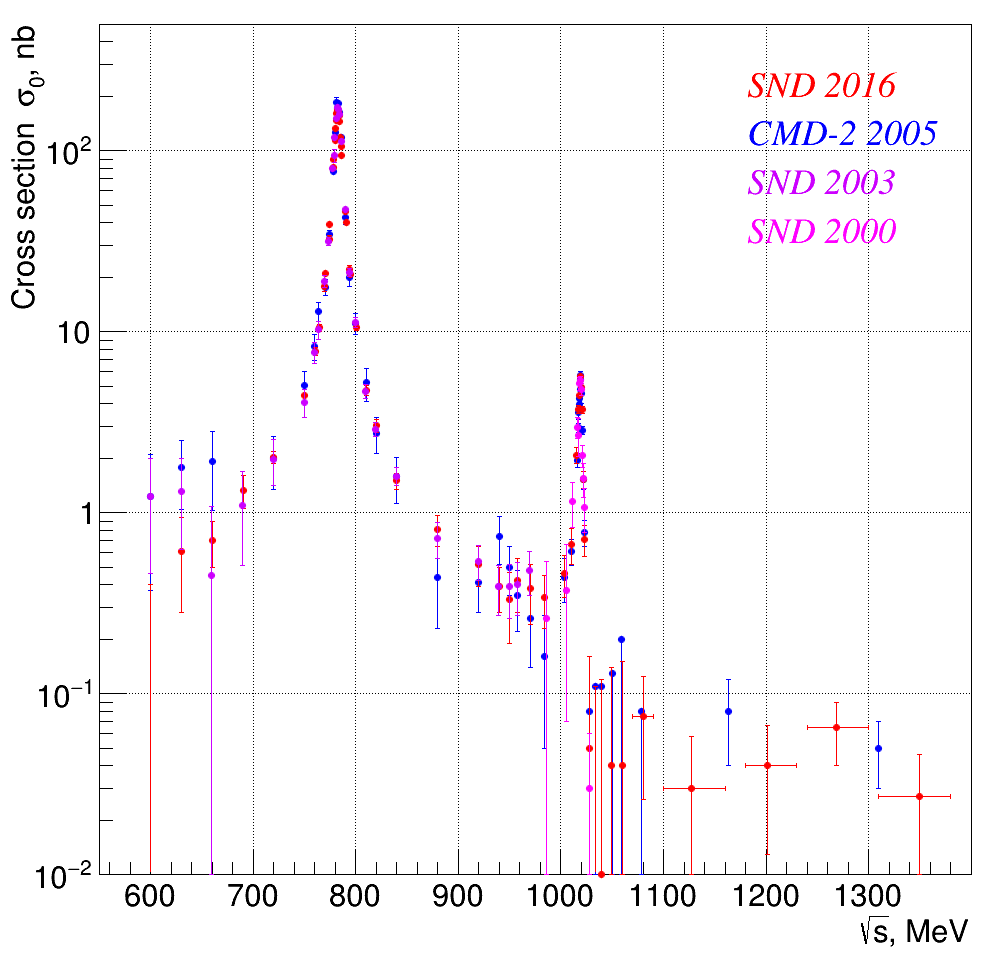
\includegraphics[width=\textwidth]{img/cs_pi0g_550_1400.png}
		\caption{Некоторые предыдущие измерения сечения $e^+ e^- \to \pi^0 \gamma$.}\label{fig:cs_pi0g_prev}
	\end{minipage}
	\hfill
	\begin{minipage}[T]{.48\textwidth}
		\centering
		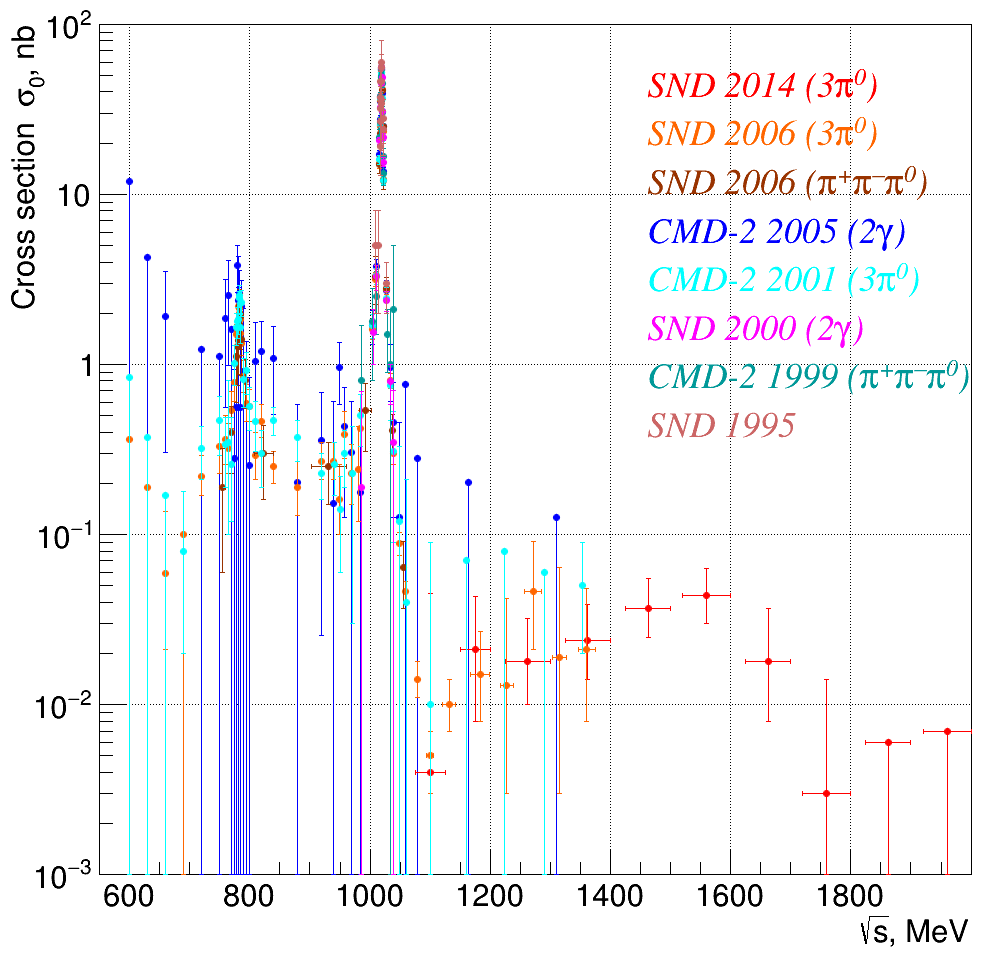
\includegraphics[width=\textwidth]{img/cs_etag_550_2000.png}
		\caption{Некоторые предыдущие измерения сечения $e^+ e^- \to \eta \gamma$.}\label{fig:cs_etag_prev}
	\end{minipage}
\end{figure}

Сечение процесса $e^+e^-\to\eta\gamma$ исследовалось во многих экспериментах.
Первые опубликованные данные появились в 1976 году из Орсая \cite{Cosme:1975rs}.
Дальнейший поток данных в основном происходит из установок Новосибирска, начиная с работы выполненной на детекторе НД \cite{Druzhinin:1984zq} и продолжая данными с КМД-2 \cite{Akhmetshin:1995vz, Akhmetshin:1999zv, Akhmetshin:2001hm, Akhmetshin:2004gw} и СНД \cite{Achasov:1997nq, Achasov:2000zd, Achasov:2006dv, Achasov:2013eli}.
Также известно измерение сечения реакции на детекторе BaBar \cite{Aubert:2006cy}.

Сечение процесса $e^+e^-\to\pi^0\gamma$ измерено несколько раз, начиная с работы в Орсаи \cite{Cosme:1975rs} и продолжая работами в Новосибирске \cite{Druzhinin:1984zq, Achasov:2000zd, Achasov:2003ed, Akhmetshin:2004gw, Achasov:2016bfr}.
